\documentclass[a4paper]{article}

\usepackage[catalan]{babel} % Language 
\usepackage{fontspec}
\usepackage[margin=2cm]{geometry}
\usepackage{float}
\usepackage[dvipsnames]{xcolor}
\usepackage{tikz}
\usepackage{pgfplots}
\usepackage{pgfplotstable}
\usepackage[hidelinks]{hyperref}
\usepackage{enumitem}
\usepackage{amsmath}
\usepackage{gensymb} % For the degree symbol
\usepackage{graphicx}
\usepackage{longtable}
\usepackage{multirow}
\usepackage{array}
\usepackage{multicol}
\usepackage{titlesec}
\usepackage{subcaption}
\usepackage{colortbl}

\usetikzlibrary{decorations.pathmorphing}
\setcounter{secnumdepth}{4}
\setcounter{tocdepth}{4}

\setlength{\parindent}{0pt}
\setlength{\parskip}{1em}

\titleformat{\paragraph}
{\normalfont\normalsize\bfseries}{\theparagraph}{1em}{}
\titlespacing*{\paragraph}
{0pt}{3.25ex plus 1ex minus .2ex}{1.5ex plus .2ex}

\pgfplotsset{
	barChart/.style={
		width=1\textwidth, height=0.5\textwidth,
		every axis plot post/.style={/pgf/number format/fixed},
		ybar=5pt,
		xtick = data,
		axis x line = bottom,
		axis y line = left,
		bar width=12pt,
		enlarge x limits = 0.2,
		visualization depends on=rawy\as\rawy, % Save the unclipped values
		after end axis/.code={ % Draw line indicating break
			\draw [ultra thick, white, decoration={snake, amplitude=1pt}, decorate] (rel axis cs:0,1.05) -- (rel axis cs:1,1.05);
		},
		nodes near coords={	\pgfmathprintnumber{\rawy} }, % Print unclipped values
		clip = false,
		x tick label style={rotate=45, anchor=east},
	}
}

\newcolumntype{R}{>{\raggedleft}p{2cm}}
\newcommand{\sectionbreak}{\clearpage}

\title{Projecte APA}
\author{Joan Marcè \and Esteve Tarragó}

\begin{document}

\begin{titlepage}
	\centering
	\vspace{1cm}
	
\includegraphics[width=0.25\textwidth]{images/logoFIB}
	\par\vspace{1cm}
	\textsc{ \LARGE Facultat d'Informàtica de Barcelona}
	\par\vspace{2cm}
	\textbf{\Huge Aprenentatge Automàtic}
	\par\vspace{2cm}
	{\LARGE Pràctica}
	\par\vspace{1em}
	{\Large Tardor curs 2016 - 2017}
	\vfill
	\begin{flushright}
		\large
		Joan Marcè Igual \par
		Esteve Tarragó Sanchis
	\end{flushright}
\end{titlepage}

\tableofcontents
\newpage

\section{Introducció}

En aquest treball s'ha de realitzar una aplicació pràctica dels diferents coneixements de \emph{Machine Learning} adquirits a classe. Així doncs, s'ha escollit un conjunt de dades per realitzar una aplicació pràctica mitjançant mètodes de classificació. 

El conjunt de dades escollit ha estat \emph{Grammatical Facial Expressions Data Set}. Aquests han estat obtinguts mitjançant una càmera \emph{Kinect} que ha enregistrat diferents punts (100) en tres dimensions de la cara de diverses persones al llarg del temps mentre realitzen una paraula en el llenguatge de signes brasiler. Aquestes expressions van combinades amb gestos amb la mà però en aquest cas només s'ha gravat la cara. Després, aquests conjunts han estat analitzats manualment per decidir quins fotogrames estan fent realment una expressió facial i quins no. 

Les dades es poden obtenir en el següent enllaç:  \url{http://archive.ics.uci.edu/ml/datasets/Grammatical+Facial+Expressions}

A part, aquestes dades també s'han usat en treballs anteriors \cite{freitas}.

\begin{figure}[H]
	\centering
	\fbox{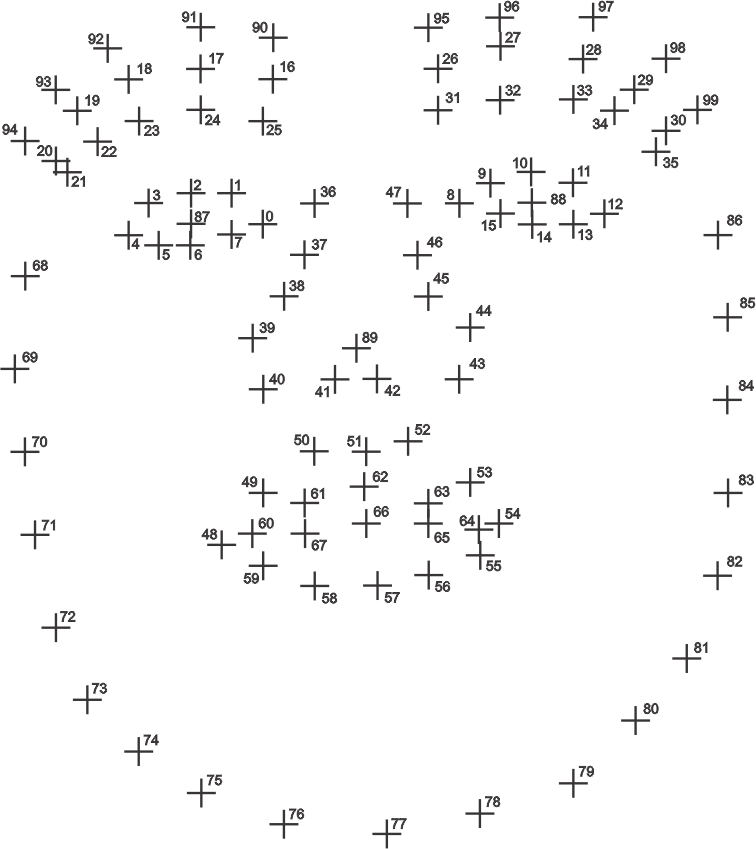
\includegraphics[width=0.6\textwidth]{images/view_points}}
	\caption{Representació dels punts de la cara que són utilitzats en la presa de dades}
\end{figure}

\section{Objectius}

L'objectiu d'aquest treball és poder decidir a partir d'una dada no usada prèviament:
\begin{enumerate}
	\item A partir de tot el conjunt de dades si s'està realitzant o no una expressió facial.
	\item En el cas en el que s'estigui realitzant una expressió facial, poder decidir de quin tipus d'expressió facial (o paraula) es tracta.
	\item Trobar quin tipus de model s'adequa millor als objectius anteriors i comprar-los entre ells.
\end{enumerate}

\section{Procés d'exploració de dades}

Les dades han estat obtingudes mitjançant una càmera Kinect RGB\cite{freitas} i el format en el que venen les dades és el següent: hi ha 9 expressions facials diferents i hi ha dos subjectes de prova. Per cada expressió facial i subjecte hi ha:
\begin{itemize}
	\item Un arxiu \verb|<subjecte>_<expressio>_datapoints.txt| que conté 1 coordenada de temps i 100 punts en 3 dimensions fent un total de 301 coordenades per arxiu.
	\item Un arxiu \verb|<subjecte>_<expressio>_targets.txt| que per a cada element de l'arxiu \verb|*_datapoints.txt| val 0 o 1 en funció de si s'està fent o no l'expressió facial a la que fa referència l'arxiu.
\end{itemize}



Donat que s'està fent classificació no s'ha considerat rellevant la coordenada de temps i, per tant, s'ha descartat. A part, s'han igualat les variàncies de totes les dades (mitjançant la rutina \verb|scale()|).

S'han realitzat dos \emph{scripts} en R. El primer és per visualitzar les dades cronològicament (\verb|loadData.R|) i el segon és per poder interpretar-les a l'hora de realitzar una classificació (\verb|clustering.R|).

En aquest cas interessa més el segon ja que és el que tracta el problema de \emph{clustering}. S'han realitzat dos tipus d'algoritmes\cite{bishop} per projectar les dades, FDA i PCA. L'\emph{script} requereix que es seleccioni primerament quina expressió (\verb|*_datapoints.txt|) es vol agafar. També cal introduir de quin punt es volen visualitzar les dades (variable \verb|point| dins de l'script). 

A continuació es mostren els resultats obtinguts amb el conjunt de dades \verb|a_affirmative_datapoints.txt| i \verb|a_affirmative_targets.txt| i el punt 60 que correspon a la part superior del llavi. Per representar les dades s'han restat les mitjanes per tal que tant els punts com la recta de projecció estiguin centrades al voltant de $(0,0)$.

\begin{longtable}{cc}
	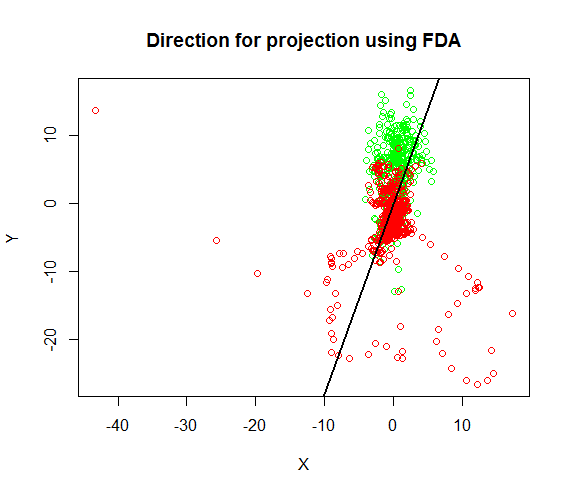
\includegraphics[width=0.45\textwidth]{images/FDA_XY} &
	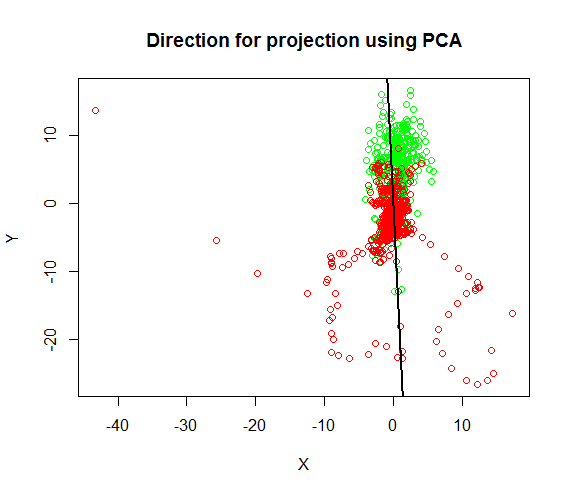
\includegraphics[width=0.45\textwidth]{images/PCA_XY} \\
	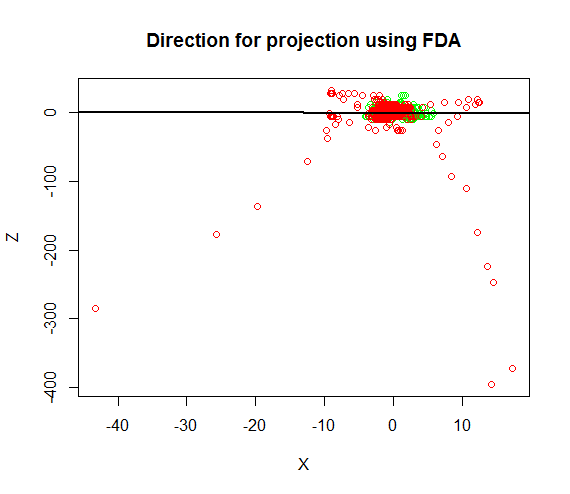
\includegraphics[width=0.45\textwidth]{images/FDA_XZ} &
	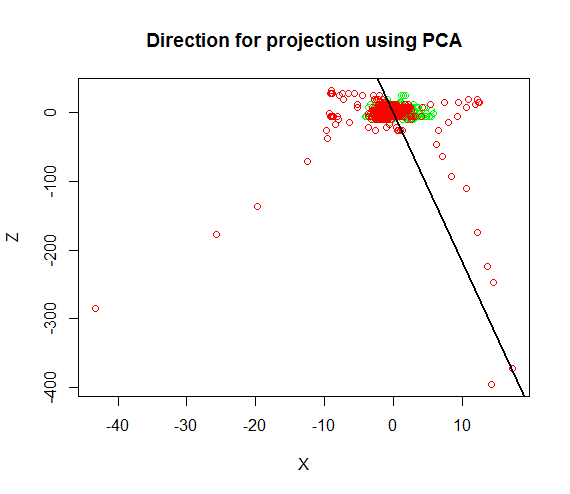
\includegraphics[width=0.45\textwidth]{images/PCA_XZ} \\
	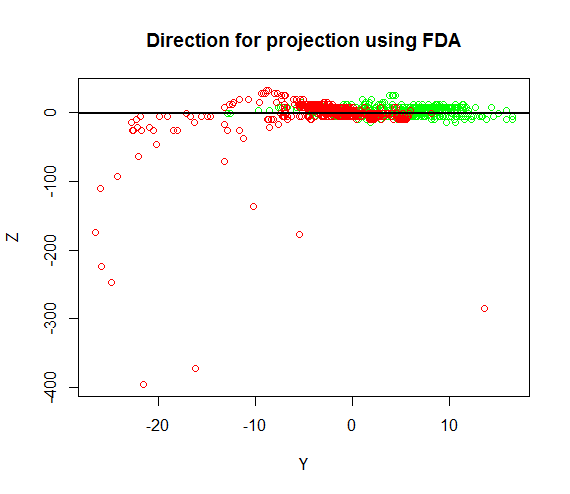
\includegraphics[width=0.45\textwidth]{images/FDA_YZ} &
	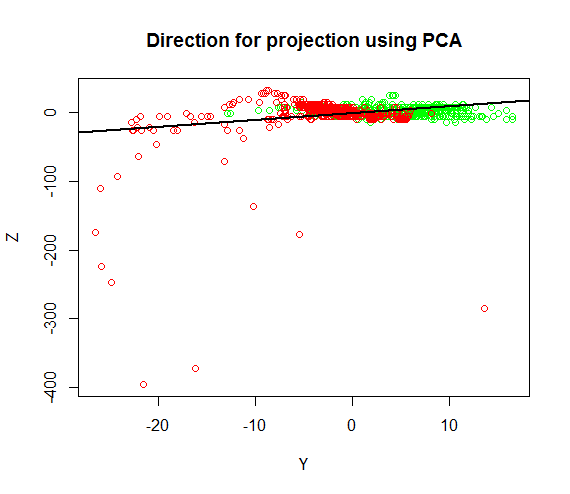
\includegraphics[width=0.45\textwidth]{images/PCA_YZ} \\
	\multicolumn{2}{c}{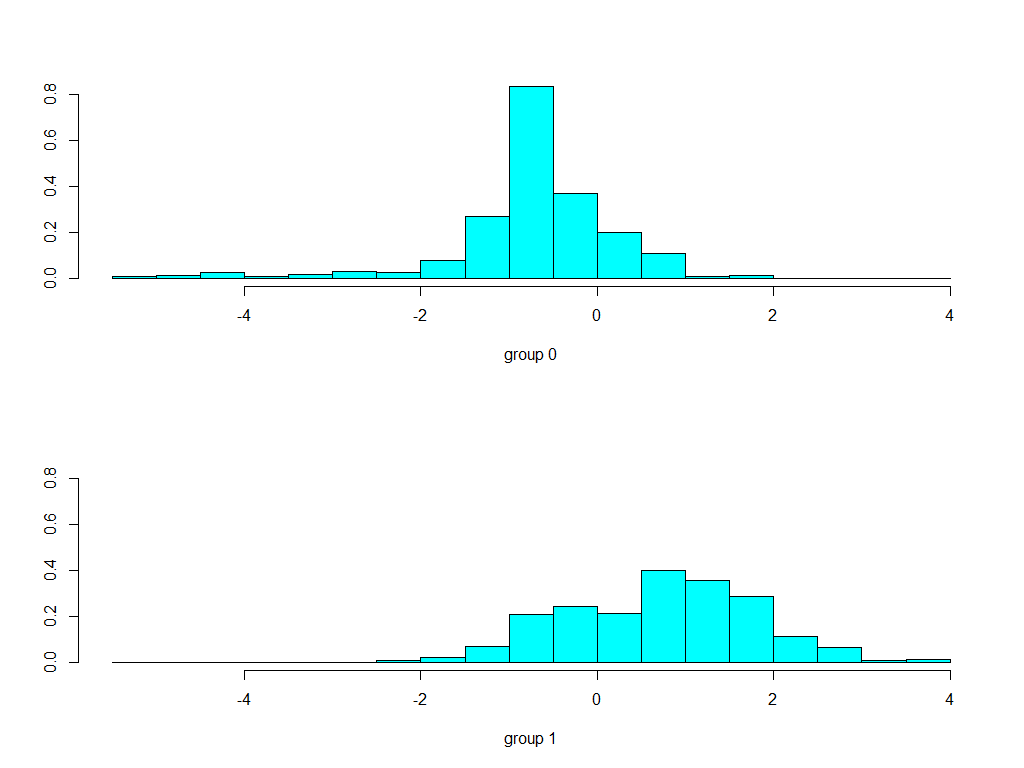
\includegraphics[width=0.8\textwidth]{images/FDA_results}}
\end{longtable}

Com es pot veure als gràfics anteriors la dada Z no permet agrupar les dades gaire bé ja que totes queden al voltant dels valors \verb|Z = 0|. Tot i així es pot veure en les dimensions $X$ i $Y$ la separació de les dades es relativament fàcil. A part també a la projecció es pot veure com queden relativament ben separades les dades.

També, donat que sembla ser viable una projecció, s'ha fet a l'script \texttt{reduceData.R} que projecta cada punt a una sola dimensió reduint l'espai de dades de 300 a 100 dimensions. Tot i així hi ha una pèrdua d'informació al fer la projecció però s'ha considerat que aquesta pèrdua d'informació és poca en comparació al guany que s'obté al reduir les dimensions.

\section{Resultats amb mètodes lineals/quadràtics}
Donat que hi ha diversos objectius en aquest treball s'han usat diferents mètodes per a poder resoldre cadascun dels objectius, han estat els següents:
\begin{itemize}
	\item Regressió logística i LDA:
	\begin{itemize}
		\item A partir de tot el conjunt de dades si s'està realitzant o no una expressió facial.
	\end{itemize}
	\item QDA i LDA:
	\begin{itemize}
		\item En el cas en el que s'estigui realitzant una expressió facial, poder decidir de quin tipus d'expressió facial (o paraula) es tracta.
	\end{itemize}
\end{itemize}

\subsection{Detecció d'expressió facial}
\subsubsection{Regressió Logística}
L'script \verb|logistic.R| realitza classificació amb regressió logística mitjançant l'ajuda de \verb|glm|. Per poder utilitzar l'script cal posar el \verb|Working Directory| a l'arrel de la carpeta subministrada i un cop es comença a executar cal escollir les dades que es volen usar per entrenar i les que es volen usar per validar. Inicialment s'havia decidit usar les dades dels arxius \verb|a_*.txt| per entrenar i les dels \verb|b_*.txt| per validar les dades tot i que això no aporta bons resultats. A continuació es pot comparar l'error entre utilitzar un sol conjunt per entrenar i usar un subconjunt de totes les dades.

En el primer experiment s'han usat totes les expressions facials d'una persona (dades contingudes a tots els arxius \verb|a_*.txt|) per a l'entrenament i per a la validació s'han usat totes les dades de l'altre persona (dades contingudes a tots els arxius \verb|b_*.txt|). Es poden veure els resultats a la \autoref{tab:reglog_training1} i la \autoref{tab:reglog_training2}.

\begin{table}[H]
	\def\arraystretch{1.5}
	\begin{subtable}[t]{0.49\textwidth}
		\centering
		\begin{tabular}{|c|rr|}
			\hline
			& \multicolumn{2}{c|}{Valor real} \\
			Valor predit & 0 & 1 \\
			\hline
			0 & 8912 & 361 \\
			1 & 242 & 4095 \\
			\hline
		\end{tabular}
		\caption{Conjunt d'entrenament. L'error és d'un 4,43\%.}
		\label{tab:reglog_training1}
	\end{subtable}
	\begin{subtable}[t]{0.49\textwidth}
		\centering
		\begin{tabular}{|c|rr|}
			\hline
			& \multicolumn{2}{c|}{Valor real} \\
			Valor predit & 0 & 1 \\
			\hline
			0 & 5725 & 2962 \\
			1 & 3180 & 2459 \\
			\hline
		\end{tabular}
		\caption{Conjunt de validació. L'error és d'un 42,87\%.}
		\label{tab:reglog_training2}
	\end{subtable}
	\caption{Valors predits al primer experiment}
\end{table}

En aquest segon experiment s'ha usat un subconjunt de totes les dades per entrenar i el complementari d'aquest per validar les dades, com es pot observar a la \autoref{tab:reglog_training4} s'obtenen millors resultats per les dades de validació respecte \autoref{tab:reglog_training2}.

\begin{table}[H]
	\def\arraystretch{1.5}
	\begin{subtable}[t]{0.49\textwidth}
		\centering
		\begin{tabular}{|c|rr|}
			\hline
			& \multicolumn{2}{c|}{Valor real} \\
			Valor predit & 0 & 1 \\
			\hline
			0 & 2306 & 543 \\
			1 &  247 & 894 \\
			\hline
		\end{tabular}
		\caption{Conjunt d'entrenament. L'error és d'un 19,8 \%.}
		\label{tab:reglog_training3}
	\end{subtable}
	\hfill
	\begin{subtable}[t]{0.49\textwidth}
		\centering
		\begin{tabular}{|c|rr|}
			\hline
			& \multicolumn{2}{c|}{Valor real} \\
			Valor predit & 0 & 1 \\
			\hline
			0 & 13914 & 3147 \\
			1 &  1592 & 5293 \\
			\hline
		\end{tabular}
		\caption{Conjunt de validació. L'error és d'un 19,79 \%.}
		\label{tab:reglog_training4}
	\end{subtable}
	\caption{Valors predits al segon experiment}
\end{table}

\subsubsection{LDA}
L'script \verb|LDA_si_no.R| realitza classificació amb \emph{lda} mitjançant l'ajuda de \verb|lda|. Per poder utilitzar l'script cal posar el \verb|Working Directory| a l'arrel de la carpeta subministrada i un cop es comença a executar cal escollir les dades que es volen usar. 
 
En el primer experiment s'han usat totes les expressions facials d'una persona (dades contingudes a tots els arxius \verb|a_*.txt|) per a l'entrenament i per a la validació s'han usat totes les dades de l'altre persona (dades contingudes a tots els arxius \verb|b_*.txt|). Es poden veure els resultats a la \autoref{tab:lda_yes_no1} i la 	\autoref{tab:lda_yes_no2}.

\begin{table}[H]
	\def\arraystretch{1.5}
	\begin{subtable}[t]{0.49\textwidth}
		\centering
		\begin{tabular}{|c|rr|}
			\hline
			& \multicolumn{2}{c|}{Valor real} \\
			Valor predit & 0 & 1 \\
			\hline
			0 & 8876 & 459 \\
			1 & 278 & 3997 \\
			\hline
		\end{tabular}
		\caption{Conjunt d'entrenament. L'error és d'un 5,42\%.}
		\label{tab:lda_yes_no1}
	\end{subtable}
	\hfill
	\begin{subtable}[t]{0.49\textwidth}
		\centering
		\begin{tabular}{|c|rr|}
			\hline
			& \multicolumn{2}{c|}{Valor real} \\
			Valor predit & 0 & 1 \\
			\hline
			0 & 5018 & 2317 \\
			1 & 3887 & 3104 \\
			\hline
		\end{tabular}
		\caption{Conjunt de validació. L'error és d'un 43,31\%.}
		\label{tab:lda_yes_no2}
	\end{subtable}
	\caption{Valors predits al primer experiment}
\end{table}

En aquest segon experiment s'ha usat un subconjunt de totes les dades per entrenar i el complementari d'aquest per validar les dades, com es pot observar a la \autoref{tab:lda_yes_no4} s'obtenen millors resultats per les dades de validació.

\begin{table}[H]
	\def\arraystretch{1.5}
	\begin{subtable}[t]{0.49\textwidth}
		\centering
		\begin{tabular}{|c|rr|}
			\hline
			& \multicolumn{2}{c|}{Valor real} \\
			Valor predit & 0 & 1 \\
			\hline
			0 & 2410 & 564 \\
			1 &  194 & 822 \\
			\hline
		\end{tabular}
		\caption{Conjunt d'entrenament. L'error és d'un 19 \%.}
		\label{tab:lda_yes_no3}
	\end{subtable}
	\hfill
	\begin{subtable}[t]{0.49\textwidth}
		\centering
		\begin{tabular}{|c|rr|}
			\hline
			& \multicolumn{2}{c|}{Valor real} \\
			Valor predit & 0 & 1 \\
			\hline
			0 & 12334 & 3036 \\
			1 &  1223 & 4359 \\
			\hline
		\end{tabular}
		\caption{Conjunt de validació. L'error és d'un 20,33 \%.}
		\label{tab:lda_yes_no4}
	\end{subtable}
	\caption{Valors predits al segon experiment}
\end{table}

\subsection{Detecció de tipus d'expressió}
\subsubsection{Tipus d'expressió}
\label{sec:tipus_expressio}
\begin{multicols}{3}
	\begin{enumerate}
		\item None 
		\item affirmative 
		\item conditional 
		\item doubt question 
		\item emphasis 
		\item negative 
		\item relative 
		\item topics 
		\item wh question 
		\item yn question
	\end{enumerate}
\end{multicols}

\subsubsection{LDA}

L’script \verb|LDA_K.R|  obté un model LDA i a continuació testeja el model mitjançant cross-validation i aplicant-lo a un altre subjecte.

Els resultats obtinguts son oposats. Això ens indica que hi ha fortes diferències entre els les expressions de ambdues persones exceptuant la expressió condicional que obté un un error molt reduït en comparació a la resta d’expressions.

També destaca que les expressions de afirmació s’han classificat com a èmfasis majoritàriament i viceversa. Això podria indicar que la persona B i la A tenen les expressions de èmfasis i afirmació invertides.

\begin{table}[H]
	\centering
	\def\arraystretch{1.2}
	\begin{tabular}{|c|rrrrrrrrrr|}
		\hline
		& \multicolumn{10}{c|}{Valor real} \\
		Valor predit & 1 & 2 & 3 & 4 & 5 & 6 & 7 & 8 & 9 & 10 \\
		 \hline
		1 & 8626 & 61 & 22 & 67 & 26 & 57 & 35 & 42 & 40 & 40 \\
		2 & 98 & 353 & 4 & 3 & 1 & 3 & 2 & 1 & 0 & 3 \\
		3 & 45 & 0 & 497 & 10 & 2 & 3 & 0 & 1 & 0 & 3 \\
		4 & 43 & 0 & 4 & 372 & 2 & 2 & 1 & 1 & 0 & 5 \\
		5 & 25 & 0 & 2 & 5 & 295 & 5 & 0 & 1 & 0 & 0 \\
		6 & 66 & 0 & 4 & 6 & 0 & 448 & 0 & 1 & 0 & 2 \\
		7 & 49 & 0 & 4 & 3 & 1 & 2 & 602 & 1 & 0 & 5 \\
		8 & 44 & 0 & 5 & 5 & 1 & 1 & 2 & 311 & 0 & 3 \\
		9 & 98 & 0 & 3 & 11 & 0 & 2 & 1 & 1 & 569 & 1 \\
		10 & 60 & 0 & 3 & 9 & 2 & 5 & 1 & 0 & 0 & 470 \\
		\hline
	\end{tabular}
	\caption{Resultats obtinguts a l'usar cross-validation. Error total 8\%.}
\end{table}


\begin{figure}[H]
	\centering
	\begin{tikzpicture}
		\begin{axis}[
				barChart,
				ymin = 0, ymax = 700,
				restrict y to domain*=0:800,
				xticklabels from table = {data/lda_k_train.csv}{category},
			]
			\addplot table[x expr=\coordindex, y=hit] {data/lda_k_train.csv};
			\addplot table[x expr=\coordindex, y=miss] {data/lda_k_train.csv};
			\legend{Hit, Miss}
		\end{axis}
	\end{tikzpicture}
	\captionsetup{width=0.8\textwidth}
	\caption{Gràfic comparatiu de l'error d'entrenament en funció del tipus d'expressió facial utilitzant LDA.}
\end{figure}

\begin{table}[H]
	\centering
	\def\arraystretch{1.2}
	\begin{tabular}{|c|rrrrrrrrrr|}
		\hline
		& \multicolumn{10}{c|}{Valor real} \\
		Valor predit & 1 & 2 & 3 & 4 & 5 & 6 & 7 & 8 & 9 & 10 \\
		\hline
		1 & 8 & 0 & 0 & 0 & 1 & 0 & 0 & 0 & 0 & 0\\
		2 & 855 & 2 & 0 & 65 & \textcolor{Orange}{349} & 0 & 14 & 0 & 21 & 137\\
		3 & 1393 & 0 & 554 & 0 & 27 & 6 & 0 & 0 & 3 & 0\\
		4 & 182 & 0 & 35 & 74 & 0 & 0 & 0 & 0 & 0 & 9\\
		5 & 3172 & \textcolor{Orange}{526} & 0 & 518 & 0 & 586 & 0 & 465 & 358 & 88\\
		6 & 360 & 0 & 0 & 3 & 0 & 0 & 0 & 0 & 72 & 73\\
		7 & 954 & 0 & 0 & 46 & 72 & 120 & 0 & 0 & 24 & 325\\
		8 & 8 & 0 & 0 & 17 & 82 & 0 & 0 & 1 & 2 & 0\\
		9 & 520 & 0 & 0 & 0 & 0 & 0 & 66 & 0 & 0 & 14\\
		10 & 1453 & 0 & 0 & 57 & 0 & 0 & 470 & 1 & 69 & 69\\
		\hline
	\end{tabular}
\captionsetup{width=0.8\textwidth}
	\caption{Resultats obtinguts al validar les dades amb una altra persona, error total 95\%. Les expressions es poden veure a la \autoref{sec:tipus_expressio}.}
\end{table}

\begin{figure}[H]
	\centering
	\begin{tikzpicture}
		\begin{axis}[
				barChart,
				ymin = 0, ymax = 850,
				restrict y to domain*=0:950,
				xticklabels from table = {data/lda_k_valid.csv}{category},
			]
			\addplot table[x expr=\coordindex, y=hit] {data/lda_k_valid.csv};
			\addplot table[x expr=\coordindex, y=miss] {data/lda_k_valid.csv};
			\legend{Hit, Miss}
		\end{axis}
	\end{tikzpicture}
	\captionsetup{width=0.8\textwidth}
	\caption{Gràfic comparatiu de l'error de validació en funció del tipus d'expressió facial utilitzant LDA.}
\end{figure}

\subsubsection{QDA}
L’script \verb|QDA_K.R|  obté un model QDA i a continuació testeja el model mitjançant cross-validation i aplicant-lo a un altre subjecte.


En comparació amb el LDA podem veure un error molt major alhora de predir les no expressions. També veiem que l’error a l’hora de predir quan s’esta fent una expressió es molt menor que en el LDA exceptuant l’expressió d’emphasis que LDA la categoritza millor

\begin{table}[H]
	\centering
	\def\arraystretch{1.2}
	\begin{tabular}{|c|rrrrrrrrrr|}
		\hline
		& \multicolumn{10}{c|}{Valor real} \\
		Valor predit & 1 & 2 & 3 & 4 & 5 & 6 & 7 & 8 & 9 & 10 \\
		\hline
		1 & 3131 & 0 & 0 & 2 & 23 & 0 & 0 & 53 & 0 & 1 \\
		2 & 572 & 409 & 0 & 0 & 0 & 0 & 0 & 0 & 0 & 0 \\
		3 & 850 & 0 & 510 & 0 & 0 & 0 & 0 & 0 & 0 & 0 \\
		4 & 582 & 0 & 0 & 461 & 0 & 0 & 0 & 0 & 0 & 0 \\
		5 & 0 & 0 & 0 & 0 & 4 & 0 & 0 & 0 & 0 & 0 \\
		6 & 541 & 0 & 0 & 0 & 0 & 492 & 0 & 0 & 0 & 0 \\
		7 & 1204 & 0 & 0 & 0 & 0 & 0 & 621 & 0 & 0 & 0 \\
		8 & 196 & 0 & 0 & 0 & 0 & 0 & 0 & 202 & 0 & 0 \\
		9 & 623 & 0 & 0 & 0 & 0 & 0 & 0 & 0 & 605 & 0 \\
		10 & 782 & 0 & 0 & 0 & 0 & 0 & 0 & 0 & 0 & 509 \\
		\hline
	\end{tabular}
	\captionsetup{width=0.8\textwidth}
	\caption{Resultats obtinguts al validar les dades amb cross-validation, error total 43\%. Les expressions es poden veure a \autoref{sec:tipus_expressio}.}
\end{table}

\begin{figure}[H]
	\centering
	\begin{tikzpicture}
		\begin{axis}[
				barChart,
				ymin = 0, ymax = 3300,
				restrict y to domain*=0:3600,
				xticklabels from table = {data/qda_k_train.csv}{category},
			]
			\addplot table[x expr=\coordindex, y=hit] {data/qda_k_train.csv};
			\addplot table[x expr=\coordindex, y=miss] {data/qda_k_train.csv};
			\legend{Hit, Miss}
		\end{axis}
	\end{tikzpicture}
	\captionsetup{width=0.8\textwidth}
	\caption{Gràfic comparatiu de l'error d'entrenament en funció del tipus d'expressió facial utilitzant QDA.}
\end{figure}

Quan s'utilitza un altre individu per validar les dades, totes es prediuen amb sortida \emph{None} per tant aquest model no ens permet extrapolar res tot hi tenir un error total menor (35\%). Es podria dir que el individu B es menys expressiu que l’individu A en aquest model ja que totes les seves expressions es categoritzen com a \emph{no expressió}.

\section{Resultats amb mètodes no lineals}
En el cas dels mètodes no lineals s'usaran Xarxes neuronals i Màquines de Vector Suport per a complir tots els objectius.

\subsection{Detecció d'expressió facial}
\subsubsection{Xarxes neuronals}

Per poder classificar mitjançant Xarxes Neuronals s'ha creat l'script \verb|neural_si_no.R| que utilitza la rutina \verb|train()| amb el mètode \verb|nnet| per tal de trobar el millor paràmetre per a la xarxa neuronal. Per verificar les dades de \verb|train()| s'usa \emph{Cross-Validation} amb 4 grups. Els resultats obtinguts han estat els següents:

\begin{table}[H]
	\centering
	\def\arraystretch{1.2}
	\begin{tabular}{|rrrr|}
		\hline
		size & decay & Accuracy & Kappa \\
		\hline
		13 & 0,00 & 0,7862118 & 0,5268094 \\
		13 & 0,01 & 0,7959902 & 0,5506152 \\
		13 & 0,10 & 0,8200551 & 0,5999062 \\
		15 & 0,00 & 0,7837126 & 0,5273864 \\
		15 & 0,01 & 0,7974985 & 0,5539709 \\
		15 & 0,10 & 0,8265744 & 0,6134527 \\
		17 & 0,00 & 0,7899759 & 0,5381721 \\
		17 & 0,01 & 0,7947369 & 0,5475432 \\
		17 & 0,10 & 0,8152878 & 0,5905086 \\
		19 & 0,00 & 0,7954869 & 0,5497133 \\
		19 & 0,01 & 0,8035120 & 0,5661520 \\
		\rowcolor{Orange!40}
		19 & 0,10 & 0,8308307 & 0,6229008 \\
		21 & 0,00 & 0,7879726 & 0,5345097 \\
		21 & 0,01 & 0,8095230 & 0,5771349 \\
		21 & 0,10 & 0,8270699 & 0,6155558 \\
		\hline
	\end{tabular}
	\captionsetup{width=0.6\textwidth}
	\caption{Valors retornats per la rutina \texttt{train()} indicant la precisió del model (més és millor) i els paràmetres \texttt{size} i \texttt{decay} usats.}
	\label{tab:nnet_yes_no}
\end{table}

Com es pot observar a la \autoref{tab:nnet_yes_no} els millors paràmetres per a la xarxa neuronal són $size = 19$ i $decay = 0,1$. Amb aquests paràmetres s'obtenen els següents resultats.

\begin{table}[H]
	\def\arraystretch{1.5}
	\begin{subtable}[t]{0.49\textwidth}
		\centering
		\begin{tabular}{|c|rr|}
			\hline
			& \multicolumn{2}{c|}{Valor real} \\
			Valor predit & 0 & 1 \\
			\hline
			0 & 2577 & 57 \\
			1 &   27 & 1329 \\
			\hline
		\end{tabular}
		\caption{Conjunt d'entrenament. L'error és d'un 2,11 \%.}
		\label{tab:nnet_yes_no1}
	\end{subtable}
	\hfill
	\begin{subtable}[t]{0.49\textwidth}
		\centering
		\begin{tabular}{|c|rr|}
			\hline
			& \multicolumn{2}{c|}{Valor real} \\
			Valor predit & 0 & 1 \\
			\hline
			0 & 13576 & 2078 \\
			1 &  1879 & 6413 \\
			\hline
		\end{tabular}
		\caption{Conjunt de validació. L'error és d'un 16,52 \%.}
		\label{tab:nnet_yes_no2}
	\end{subtable}
	\caption{Valors predits amb la xarxa neuronal}
\end{table}

\subsubsection{Màquines de Vectors Suport}
\paragraph{Lineals}

Per poder classificar mitjançant Màquines de Vector Suport s’ha creat l’script \verb|SVM_si_no.R| que utilitza la rutina \verb|train()| amb el mètode \verb|nnet| per tal de trobar el millor paràme	tre per a la xarxa neuronal. Per verificar les dades de \verb|train()| s’usa Cross-Validation amb 4 grups. Els resultats obtinguts han estat els següents: 

\begin{table}[H]
	\centering
	\def\arraystretch{1.2}
	\begin{tabular}{|rrr|}
		\hline
		C & Accuracy & Kappa \\
		\hline
		1 & 0,7967429 & 0,5260806 \\
		25 & 0,7992505 & 0,5352465 \\
		\rowcolor{Orange!40}
		50 & 0,8002525 & 0,5381296 \\
		75 & 0,7995017 & 0,5396425 \\
		100 & 0,7989995 & 0,5386959 \\
		\hline
	\end{tabular}
\end{table}

\begin{table}[H]
	\def\arraystretch{1.5}
	\begin{subtable}[t]{0.49\textwidth}
		\centering
		\begin{tabular}{|c|rr|}
			\hline
			& \multicolumn{2}{c|}{Valor real} \\
			Valor predit & 0 & 1 \\
			\hline
			0 & 2365 & 509 \\
			1 &  233 & 883 \\
			\hline
		\end{tabular}
		\caption{Conjunt d'entrenament. L'error és d'un 18,6 \%.}
		\label{tab:svm_lineal_yes_no1}
	\end{subtable}
	\hfill
	\begin{subtable}[t]{0.49\textwidth}
		\centering
		\begin{tabular}{|c|rr|}
			\hline
			& \multicolumn{2}{c|}{Valor real} \\
			Valor predit & 0 & 1 \\
			\hline
			0 & 14030 & 3300 \\
			1 &  1431 & 5185 \\
			\hline
		\end{tabular}
		\caption{Conjunt de validació. L'error és d'un 19,76 \%.}
		\label{tab:svm_lineal_yes_no2}
	\end{subtable}
	\caption{Valors predits amb una màquina de vectors suport lineal}
\end{table}

\paragraph{Radial}

\begin{table}[H]
	\def\arraystretch{1.5}
	\begin{subtable}[t]{0.49\textwidth}
		\centering
		\begin{tabular}{|c|rr|}
			\hline
			& \multicolumn{2}{c|}{Valor real} \\
			Valor predit & 0 & 1 \\
			\hline
			0 & 2594 &   68 \\
			1 &    4 & 1324 \\
			\hline
		\end{tabular}
		\caption{Conjunt d'entrenament. L'error és d'un 1,8 \%.}
		\label{tab:svm_radial_yes_no1}
	\end{subtable}
	\hfill
	\begin{subtable}[t]{0.49\textwidth}
		\centering
		\begin{tabular}{|c|rr|}
			\hline
			& \multicolumn{2}{c|}{Valor real} \\
			Valor predit & 0 & 1 \\
			\hline
			0 & 14324 & 2010 \\
			1 &  1137 & 6475 \\
			\hline
		\end{tabular}
		\caption{Conjunt de validació. L'error és d'un 13,14 \%.}
		\label{tab:svm_radial_yes_no2}
	\end{subtable}
	\caption{Valors predits amb una màquina de vectors suport radial}
\end{table}

\subsection{Detecció de tipus d'expressió}
\subsubsection{Xarxes neuronals}

Per poder classificar mitjançant Xarxes Neuronals s'ha creat l'script \verb|neural_K.R| que utilitza la rutina \verb|train()| amb el mètode \verb|nnet| per tal de trobar el millor paràmetre per a la xarxa neuronal. Per verificar les dades de \verb|train()| s'usa \emph{Cross-Validation}.

\begin{table}[H]
	\centering
	\def\arraystretch{1.2}
	\begin{tabular}{|rrrr|}
		\hline
		size & decay & Accuracy & Kappa \\
		\hline
		13 & 0,01 & 0,7024945 & 0,4582371 \\
		13 & 0,10 & 0,7563778 & 0,5359380 \\
		15 & 0,01 & 0,7232956 & 0,4988062 \\
		15 & 0,10 & 0,7543884 & 0,5358015 \\
		17 & 0,01 & 0,7225496 & 0,5021978 \\
		17 & 0,10 & 0,7583979 & 0,5492146 \\
		19 & 0,01 & 0,7190431 & 0,5001007 \\
		19 & 0,10 & 0,7659132 & 0,5608208 \\
		21 & 0,01 & 0,7177959 & 0,5018095 \\
		21 & 0,10 & 0,7696662 & 0,5735675 \\
		23 & 0,01 & 0,7077666 & 0,4891685 \\
		23 & 0,10 & 0,7786963 & 0,5862649 \\
		25 & 0,01 & 0,7177911 & 0,4999727 \\
		\rowcolor{Orange!40}
		25 & 0,10 & 0,7711760 & 0,5728318 \\
		27 & 0,01 & 0,7255627 & 0,5074409 \\
		27 & 0,10 & 0,7687221 & 0,6025761 \\
		\hline
	\end{tabular}
	\captionsetup{width=0.6\textwidth}
	\caption{Valors retornats per la rutina \texttt{train()} indicant la precisió del model (més és millor) i els paràmetres \texttt{size} i \texttt{decay} usats.}
	\label{tab:nnet_k}
\end{table}

Com es pot observar a la \autoref{tab:nnet_k} els millors paràmetres per a la xarxa neuronal són $size = 25$ i $decay = 0,1$. Amb aquests paràmetres s'obtenen els següents resultats:

\begin{table}[H]
	\centering
	\def\arraystretch{1.2}
	\begin{tabular}{|c|rrrrrrrrrr|}
		\hline
		& \multicolumn{10}{c|}{Valor real} \\
		Valor predit & 1 & 2 & 3 & 4 & 5 & 6 & 7 & 8 & 9 & 10 \\
		\hline
		1 & 2613 & 10 & 7 & 10 & 5 & 7 & 11 & 5 & 16 & 14 \\
		2 & 2 & 117 & 0 & 1 & 1 & 0 & 1 & 0 & 0 & 2 \\
		3 & 1 & 0 & 151 & 1 & 0 & 0 & 0 & 1 & 0 & 1 \\
		4 & 3 & 0 & 0 & 145 & 0 & 0 & 0 & 0 & 1 & 0 \\
		5 & 0 & 1 & 0 & 0 & 100 & 0 & 0 & 1 & 0 & 0 \\
		6 & 0 & 0 & 0 & 0 & 0 & 167 & 0 & 0 & 0 & 0 \\
		7 & 0 & 3 & 3 & 0 & 2 & 1 & 148 & 0 & 0 & 1 \\
		8 & 1 & 0 & 0 & 0 & 0 & 0 & 0 & 95 & 0 & 0 \\
		9 & 2 & 0 & 0 & 0 & 0 & 0 & 0 & 0 & 170 & 0 \\
		10 & 1 & 1 & 3 & 0 & 0 & 0 & 1 & 0 & 0 & 163 \\
		\hline
	\end{tabular}
	\caption{Resultats obtinguts amb les dades d'entrenament. Error total 3,03\%}
	\label{tab:nnet_k1}
\end{table}

\begin{figure}[H]
	\centering
	\begin{tikzpicture}
		\begin{axis}[
				barChart,
				ymin = 0, ymax = 200,
				restrict y to domain*=0:230,
				xticklabels from table = {data/nnet_k_train.csv}{category},
			]
			\addplot table[x expr=\coordindex, y=hit] {data/nnet_k_train.csv};
			\addplot table[x expr=\coordindex, y=miss] {data/nnet_k_train.csv};
			\legend{Hit, Miss}
		\end{axis}
	\end{tikzpicture}
	\captionsetup{width=0.8\textwidth}
	\caption{Gràfic comparatiu de l'error d'entrenament en funció del tipus d'expressió facial utilitzant una xarxa neuronal.}
\end{figure}

\begin{table}[H]
	\centering
	\def\arraystretch{1.2}
	\begin{tabular}{|c|rrrrrrrrrr|}
		\hline
		& \multicolumn{10}{c|}{Valor real} \\
		Valor predit & 1 & 2 & 3 & 4 & 5 & 6 & 7 & 8 & 9 & 10 \\
		\hline
		1 & 13945 & 270 & 215 & 364 & 131 & 358 & 191 & 170 & 314 & 290 \\
		2 & 201 & 336 & 19 & 24 & 47 & 28 & 23 & 9 & 13 & 47 \\
		3 & 146 & 41 & 584 & 6 & 36 & 24 & 43 & 22 & 18 & 23 \\
		4 & 167 & 8 & 22 & 639 & 5 & 19 & 4 & 13 & 8 & 17 \\
		5 & 105 & 25 & 32 & 7 & 367 & 20 & 29 & 14 & 5 & 8 \\
		6 & 254 & 14 & 19 & 17 & 18 & 553 & 3 & 14 & 14 & 14 \\
		7 & 140 & 43 & 21 & 23 & 67 & 13 & 678 & 51 & 3 & 10 \\
		8 & 84 & 15 & 14 & 2 & 41 & 16 & 41 & 425 & 6 & 4 \\
		9 & 267 & 15 & 8 & 6 & 16 & 24 & 3 & 2 & 586 & 24 \\
		10 & 127 & 43 & 39 & 26 & 25 & 10 & 18 & 5 & 4 & 62 \\
		\hline
	\end{tabular}
	\caption{Resultats obtinguts amb les dades de validació. Error total 21,73\%}
	\label{tab:nnet_k2}
\end{table}

\begin{figure}[H]
	\centering
	\begin{tikzpicture}
	\begin{axis}[
			barChart,
			ymin = 0, ymax = 1550,
			restrict y to domain*=0:1700,
			xticklabels from table = {data/nnet_k_valid.csv}{category},
		]
		\addplot table[x expr=\coordindex, y=hit] {data/nnet_k_valid.csv};
		\addplot table[x expr=\coordindex, y=miss] {data/nnet_k_valid.csv};
		\legend{Hit, Miss}
	\end{axis}
	\end{tikzpicture}
	\captionsetup{width=0.8\textwidth}
	\caption{Gràfic comparatiu de l'error de validació en funció del tipus d'expressió facial utilitzant una xarxa neuronal.}
\end{figure}

\subsubsection{Màquines de Vectors Suport}
\paragraph{Lineal}

\begin{table}[H]
	\centering
	\def\arraystretch{1.2}
	\begin{tabular}{|rrr|}
		\hline
		C & Accuracy & Kappa \\
		8 & 0,7593957 & 0,4902876 \\
		\rowcolor{Orange!40}
		9 & 0,7616539 & 0,4961347 \\
		10 & 0,7606533 & 0,4938614 \\
		\hline
	\end{tabular}
\end{table}

\begin{table}[H]
	\centering
	\def\arraystretch{1.2}
	\begin{tabular}{|c|rrrrrrrrrr|}
		\hline
		& \multicolumn{10}{c|}{Valor real} \\
		Valor predit & 1 & 2 & 3 & 4 & 5 & 6 & 7 & 8 & 9 & 10 \\
		\hline
		1 & 2532 & 85 & 63 & 56 & 39 & 94 & 69 & 44 & 122 & 75 \\
		2 & 3 & 46 & 0 & 0 & 0 & 0 & 0 & 0 & 0 & 0 \\
		3 & 10 & 0 & 100 & 0 & 0 & 1 & 0 & 0 & 0 & 0 \\
		4 & 10 & 2 & 0 & 120 & 0 & 0 & 1 & 0 & 0 & 1 \\
		5 & 4 & 4 & 1 & 0 & 75 & 2 & 1 & 0 & 0 & 0 \\
		6 & 1 & 0 & 0 & 0 & 1 & 75 & 0 & 0 & 0 & 0 \\
		7 & 6 & 1 & 1 & 0 & 2 & 0 & 99 & 4 & 0 & 1 \\
		8 & 4 & 0 & 1 & 1 & 0 & 1 & 0 & 70 & 0 & 0 \\
		9 & 0 & 0 & 0 & 0 & 0 & 1 & 0 & 0 & 42 & 0 \\
		10 & 4 & 2 & 0 & 2 & 0 & 0 & 2 & 0 & 0 & 109 \\
		\hline
	\end{tabular}
	\caption{Resultats obtinguts amb les dades d'entrenament. Error total 18,10 \%}
	\label{tab:svm_lineal_k1}
\end{table}

\begin{figure}[H]
	\centering
	\begin{tikzpicture}
		\begin{axis}[
				barChart,
				ymin = 0, ymax = 150,
				restrict y to domain*=0:170,
				xticklabels from table = {data/svm_lineal_k_train.csv}{category},
			]
			\addplot table[x expr=\coordindex, y=hit] {data/svm_lineal_k_train.csv};
			\addplot table[x expr=\coordindex, y=miss] {data/svm_lineal_k_train.csv};
			\legend{Hit, Miss}
		\end{axis}
	\end{tikzpicture}
	\captionsetup{width=0.8\textwidth}
	\caption{Gràfic comparatiu de l'error d'entrenament en funció del tipus d'expressió facial utilitzant una SVM lineal.}
\end{figure}

\begin{table}[H]
	\centering
	\def\arraystretch{1.2}
	\begin{tabular}{|c|rrrrrrrrrr|}
		\hline
		& \multicolumn{10}{c|}{Valor real} \\
		Valor predit & 1 & 2 & 3 & 4 & 5 & 6 & 7 & 8 & 9 & 10 \\
		\hline
		1 & 14964 & 511 & 389 & 499 & 308 & 668 & 407 & 281 & 844 & 75 \\
		2 & 13 & 171 & 3 & 16 & 5 & 4 & 23 & 12 & 2 & 0 \\
		3 & 94 & 14 & 503 & 6 & 63 & 13 & 18 & 15 & 3 & 0 \\
		4 & 90 & 8 & 7 & 523 & 4 & 23 & 30 & 2 & 4 & 1 \\
		5 & 72 & 38 & 24 & 3 & 309 & 17 & 9 & 2 & 5 & 0 \\
		6 & 77 & 3 & 8 & 3 & 9 & 307 & 1 & 0 & 12 & 0 \\
		7 & 51 & 20 & 18 & 10 & 25 & 10 & 518 & 54 & 1 & 1 \\
		8 & 44 & 14 & 10 & 10 & 5 & 12 & 5 & 342 & 1 & 0 \\
		9 & 26 & 2 & 2 & 0 & 0 & 12 & 1 & 0 & 121 & 0 \\
		10 & 54 & 21 & 7 & 22 & 16 & 0 & 10 & 1 & 1 & 109 \\
		\hline
	\end{tabular}
	\caption{Resultats obtinguts amb les dades de validació. Error total 23,92 \%}
	\label{tab:svm_lineal_k2}
\end{table}

\begin{figure}[H]
	\centering
	\begin{tikzpicture}
	\begin{axis}[
				barChart,
				ymin = 0, ymax = 950,
				restrict y to domain*=0:1150,
				xticklabels from table = {data/svm_lineal_k_valid.csv}{category},
			]
			\addplot table[x expr=\coordindex, y=hit] {data/svm_lineal_k_valid.csv};
			\addplot table[x expr=\coordindex, y=miss] {data/svm_lineal_k_valid.csv};
			\legend{Hit, Miss}
		\end{axis}
	\end{tikzpicture}
	\captionsetup{width=0.8\textwidth}
	\caption{Gràfic comparatiu de l'error de validació en funció del tipus d'expressió facial utilitzant una SVM lineal.}
\end{figure}

\paragraph{Radial}

\begin{table}[H]
	\centering
	\def\arraystretch{1.2}
	\begin{tabular}{|rrrr|}
		\hline
		C & sigma & Accuracy & Kappa \\
		\hline
		15 & 0,01 & 0,8022794 & 0,5985588 \\
		15 & 0,05 & 0,8215548 & 0,6525660 \\
		15 & 0,10 & 0,8107551 & 0,6292849 \\
		16 & 0,01 & 0,8057839 & 0,6078905 \\
		16 & 0,05 & 0,8208035 & 0,6519884 \\
		16 & 0,10 & 0,8095032 & 0,6270414 \\
		17 & 0,01 & 0,8075283 & 0,6127379 \\
		\rowcolor{Orange!40}
		17 & 0,05 & 0,8220473 & 0,6550542 \\
		17 & 0,10 & 0,8092501 & 0,6266172 \\
		\hline
	\end{tabular}
\end{table}

\begin{table}[H]
	\centering
	\def\arraystretch{1.2}
	\begin{tabular}{|c|rrrrrrrrrr|}
		\hline
		& \multicolumn{10}{c|}{Valor real} \\
		Valor predit & 1 & 2 & 3 & 4 & 5 & 6 & 7 & 8 & 9 & 10 \\
		\hline
		1 & 2570 & 20 & 13 & 18 & 4 & 6 & 13 & 3 & 27 & 14 \\
		2 & 0 & 119 & 0 & 0 & 0 & 0 & 0 & 0 & 0 & 0 \\
		3 & 0 & 0 & 153 & 0 & 0 & 0 & 0 & 0 & 0 & 0 \\
		4 & 2 & 0 & 0 & 160 & 0 & 0 & 0 & 0 & 0 & 0 \\
		5 & 0 & 0 & 0 & 0 & 112 & 0 & 0 & 0 & 0 & 0 \\
		6 & 0 & 0 & 0 & 0 & 0 & 168 & 0 & 0 & 0 & 0 \\
		7 & 0 & 1 & 0 & 0 & 1 & 0 & 159 & 0 & 0 & 0 \\
		8 & 0 & 0 & 0 & 0 & 0 & 0 & 0 & 115 & 0 & 0 \\
		9 & 0 & 0 & 0 & 0 & 0 & 0 & 0 & 0 & 137 & 0 \\
		10 & 2 & 0 & 0 & 1 & 0 & 0 & 0 & 0 & 0 & 172 \\
		\hline
	\end{tabular}
	\caption{Resultats obtinguts amb les dades d'entrenament. Error total 3,13 \%}
	\label{tab:svm_radial_k1}
\end{table}

\begin{figure}[H]
	\centering
	\begin{tikzpicture}
		\begin{axis}[
				barChart,
				ymin = 0, ymax = 200,
				restrict y to domain*=0:240,
				xticklabels from table = {data/svm_radial_k_train.csv}{category},
			]
			\addplot table[x expr=\coordindex, y=hit] {data/svm_radial_k_train.csv};
			\addplot table[x expr=\coordindex, y=miss] {data/svm_radial_k_train.csv};
			\legend{Hit, Miss}
		\end{axis}
	\end{tikzpicture}
	\captionsetup{width=0.8\textwidth}
	\caption{Gràfic comparatiu de l'error d'entrenament en funció del tipus d'expressió facial utilitzant una SVM lineal.}
\end{figure}

\begin{table}[H]
	\centering
	\def\arraystretch{1.2}
	\begin{tabular}{|c|rrrrrrrrrr|}
		\hline
		& \multicolumn{10}{c|}{Valor real} \\
		Valor predit & 1 & 2 & 3 & 4 & 5 & 6 & 7 & 8 & 9 & 10 \\
		\hline
		1 & 14829 & 375 & 286 & 307 & 208 & 434 & 201 & 156 & 440 & 335 \\
		2 & 56 & 285 & 20 & 2 & 5 & 3 & 19 & 20 & 0 & 18 \\
		3 & 73 & 13 & 553 & 13 & 25 & 15 & 57 & 22 & 8 & 13 \\
		4 & 61 & 0 & 3 & 753 & 0 & 8 & 4 & 0 & 0 & 8 \\
		5 & 46 & 28 & 37 & 0 & 438 & 5 & 21 & 17 & 1 & 2 \\
		6 & 88 & 7 & 1 & 0 & 12 & 581 & 0 & 1 & 1 & 1 \\
		7 & 68 & 50 & 45 & 4 & 36 & 0 & 678 & 55 & 2 & 8 \\
		8 & 76 & 17 & 13 & 3 & 13 & 3 & 34 & 434 & 0 & 2 \\
		9 & 105 & 5 & 2 & 3 & 5 & 13 & 2 & 0 & 542 & 5 \\
		10 & 83 & 22 & 11 & 7 & 2 & 4 & 6 & 4 & 0 & 669 \\
		\hline
	\end{tabular}
	\caption{Resultats obtinguts amb les dades de validació. Error total 17,47 \%}
	\label{tab:svm_radial_k2}
\end{table}

\begin{figure}[H]
	\centering
	\begin{tikzpicture}
		\begin{axis}[
				barChart,
				ymin = 0, ymax = 850,
				restrict y to domain*=0:950,
				xticklabels from table = {data/svm_radial_k_valid.csv}{category},
			]
			\addplot table[x expr=\coordindex, y=hit] {data/svm_radial_k_valid.csv};
			\addplot table[x expr=\coordindex, y=miss] {data/svm_radial_k_valid.csv};
			\legend{Hit, Miss}
		\end{axis}
	\end{tikzpicture}
	\captionsetup{width=0.8\textwidth}
	\caption{Gràfic comparatiu de l'error de validació en funció del tipus d'expressió facial utilitzant una SVM lineal.}
\end{figure}

\section{Model final escollit}
\section{Conclusions}
\section{Possibles extensions}
\section{Referències}

\bibliographystyle{acm}
\bibliography{bibliography}

\end{document}